
%{{第四十三回}}{第四十三回}}

\chapter{闲取乐偶攒金庆寿\hspace{.5em}不了情暂撮土为香}


{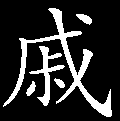
\includegraphics[width=3mm]{../Images/00005} \kaishu 了与不了在心头,迷却原来难自由。如有如无谁解得,相生相灭第传流。}

话说王夫人因见贾母那日在大观园不过着了些风寒,不是什么大病,请医生吃了两剂药也就好了,便放了心,因命凤姐来吩咐他预备给贾政带送东西。正商议着,只见贾母打发人来请,王夫人忙引着凤姐儿过来。王夫人又请问:``这会子可又觉大安些?''贾母道:``今日可大好了。方才你们送来野鸡崽子汤,我尝了一尝,倒有味儿,又吃了两块肉,心里很受用。''王夫人笑道:``这是凤丫头孝敬老太太的。算他的孝心虔,不枉了素日老太太疼他。''贾母点头笑道:``难为他想着。若是还有生的,再炸上两块,咸浸浸的,吃粥有味儿。那汤虽好,就只不对稀饭。''凤姐听了,连忙答应,命人去厨房传话。

这里贾母又向王夫人笑道:``我打发人请你来,不为别的。初二是凤丫头的生日,上两年我原早想替他做生日,偏到跟前有大事,就混过去了。今年人又齐全,料着又没事,咱们大家好生乐一日。''{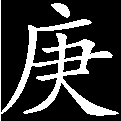
\includegraphics[width=3mm]{../Images/00004}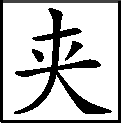
\includegraphics[width=3mm]{../Images/00012}\footnotesize \kaishu 贾母犹云``好生乐一日'',可见逐日虽乐,皆还不趁心也。所以世人无论贫富,各有愁肠,终不能时时遂心如意。此是至理,非不足语也。}王夫人笑道:``我也想着呢。既是老太太高兴,何不就商议定了?''贾母笑道:``我想往年不拘谁作生日,都是各自送各自的礼,这个也俗了,也觉生分的似的。今儿我出个新法子,又不生分,又可取笑。''王夫人忙道:``老太太怎么想着好,就是怎么样行。''贾母笑道:``我想着,咱们也学那小家子大家凑分子,{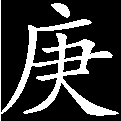
\includegraphics[width=3mm]{../Images/00004}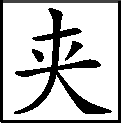
\includegraphics[width=3mm]{../Images/00012}\footnotesize \kaishu 原来凑分子是小家的事。近见多少人家红白事一出,且筹算分子之多寡,不知何说。}多少尽着这钱去办,你道好顽不好顽?''{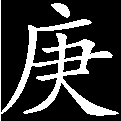
\includegraphics[width=3mm]{../Images/00004}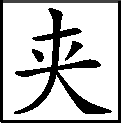
\includegraphics[width=3mm]{../Images/00012}\footnotesize \kaishu 看他写与宝钗作生日后,又偏写与凤姐作生日。阿凤何人也,岂不为彼之华诞大用一回笔墨哉?只是亏他如何想来,特写于宝钗之后,较姊妹胜而有馀;于贾母之前,较诸父母相去不远。一部书中,若一个一个只管写过生日,复成何文哉?故起用宝钗,盛用阿凤,终用贾母,各有妙文,各有妙景。馀者诸人,或一笔不写,或偶因一语带过,或丰或简,其情当理合,不表可知。岂必谆谆死笔,按数而写众人之生日哉?◇迥不犯宝钗。}王夫人笑道:``这个很好,但不知怎么凑法?''贾母听说,益发高兴起来,忙遣人去请薛姨妈、邢夫人等,{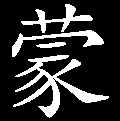
\includegraphics[width=3mm]{../Images/00006}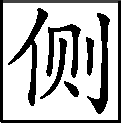
\includegraphics[width=3mm]{../Images/00011}\footnotesize \kaishu 世家之长上多犯此等``办寿也要请人''毛病。}又叫请姑娘们并宝玉,那府里珍儿媳妇并赖大家的等有头脸管事的媳妇也都叫了来。

众丫头婆子见贾母十分高兴,也都高兴,忙忙的各自分头去请的请,传的传,没顿饭的工夫,老的少的,上的下的,乌压压挤了一屋子。只薛姨妈和贾母对坐,邢夫人王夫人只坐在房门前两张椅子上,宝钗姊妹等五六个人坐在炕上,宝玉坐在贾母怀前,地下满满的站了一地。贾母忙命拿几个小杌子来,给赖大母亲等几个高年有体面的妈妈坐了。贾府风俗,年高伏侍过父母的家人,比年轻的主子还有体面,所以尤氏凤姐儿等只管地下站着,那赖大的母亲等三四个老妈妈告个罪,都坐在小杌子上了。

贾母笑着把方才一席话说与众人听了。众人谁不凑这趣儿?再也有和凤姐儿好的,有情愿这样的;有畏惧凤姐儿的,巴不得来奉承的:况且都是拿的出来的,所以一闻此言,都欣然应诺。贾母先道:``我出二十两。''薛姨妈笑道:``我随着老太太,也是二十两了。''邢夫人王夫人笑道:``我们不敢和老太太并肩,自然矮一等,每人十六两罢了。''尤氏李纨也笑道:``我们自然又矮一等,每人十二两罢。''贾母忙和李纨道:``你寡妇失业的,那里还拉你出这个钱,我替你出了罢。''{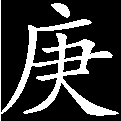
\includegraphics[width=3mm]{../Images/00004}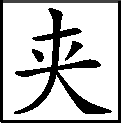
\includegraphics[width=3mm]{../Images/00012}\footnotesize \kaishu 必如是方妙。}凤姐忙笑道:``老太太别高兴,且算一算账再揽事。老太太身上已有两分呢,这会子又替大嫂子出十二两,说着高兴,一会子回想又心疼了。过后儿又说:`都是为凤丫头花了钱。'使个巧法子,哄着我拿出三四分子来暗里补上,我还做梦呢。''说的众人都笑了。贾母笑道:``依你怎么样呢?''{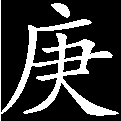
\includegraphics[width=3mm]{../Images/00004}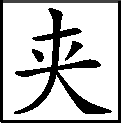
\includegraphics[width=3mm]{../Images/00012}\footnotesize \kaishu 又写阿凤一评,更妙。若一笔直下,有何趣哉?}凤姐笑道:``生日没到,我这会子已经折受的不受用了。我一个钱饶不出,惊动这些人实在不安,不如大嫂子这一分我替他出了罢了。我到了那一日多吃些东西,就享了福了。''邢夫人等听了,都说:``很是。''贾母方允了。

凤姐儿又笑道:``我还有一句话呢。我想老祖宗自己二十两,又有林妹妹宝兄弟的两分子。姨妈自己二十两,又有宝妹妹的一分子,这倒也公道。只是二位太太每位十六两,自己又少,又不替人出,这有些不公道。老祖宗吃了亏了!''贾母听了,忙笑道:``倒是我的凤丫头向着我,这说的很是。要不是你,我叫他们又哄了去了。''凤姐笑道:``老祖宗只把他姐儿两个交给两位太太,一位占一个,派多派少,每位替出一分就是了。''贾母忙说:``这很公道,就是这样。''赖大的母亲忙站起来笑说道:``这可反了!我替二位太太生气。在那边是儿子媳妇,在这边是内侄女儿,倒不向着婆婆姑娘,倒向着别人。这儿媳妇成了陌路人,内侄女儿竟成了个外侄女儿了。''说的贾母与众人都大笑起来了。{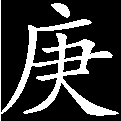
\includegraphics[width=3mm]{../Images/00004}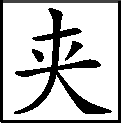
\includegraphics[width=3mm]{../Images/00012}\footnotesize \kaishu 写阿凤全副精神,虽一戏,亦人想不到之文。}

赖大之母因又问道:``少奶奶们十二两,我们自然也该矮一等了。''贾母听说,道:``这使不得。你们虽该矮一等,我知道你们这几个都是财主,果位虽低,钱却比他们多。{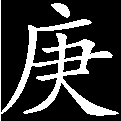
\includegraphics[width=3mm]{../Images/00004}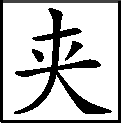
\includegraphics[width=3mm]{../Images/00012}\footnotesize \kaishu 惊魂夺魄只此一句。所以一部书全是老婆舌头,全是讽刺世事,反面春秋也。所谓``痴子弟正照风月鉴'',若单看了家常老婆舌头,岂非痴子弟乎?}你们和他们一例才使得。''众妈妈听了,连忙答应。贾母又道:``姑娘们不过应个景儿,每人照一个月的月例就是了。''又回头叫鸳鸯来,``你们也凑几个人,商议凑了来。''鸳鸯答应着,去不多时带了平儿、袭人、彩霞等还有几个小丫鬟来,也有二两的,也有一两的。贾母因问平儿:``你难道不替你主子作生日,还入在这里头?''平儿笑道:``我那个私自另外有了,这是官中的,也该出一分。''贾母笑道:``这才是好孩子。''

凤姐又笑道:``上下都全了。还有二位姨奶奶,他出不出,也问一声儿,尽到他们是理。不然,他们只当小看了他们了。''{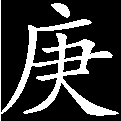
\includegraphics[width=3mm]{../Images/00004}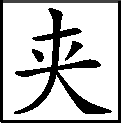
\includegraphics[width=3mm]{../Images/00012}\footnotesize \kaishu 纯写阿凤,以衬后文。}贾母听了,忙说:``可是呢,怎么倒忘了他们!只怕他们不得闲儿,叫一个丫头问问去。''说着,早有丫头去了,半日回来说道:``每位也出二两。''贾母喜道:``拿笔砚来算明,共计多少。''尤氏因悄骂凤姐道:``我把你这没足厌的小蹄子!这么些婆婆婶子来凑银子给你过生日,你还不足,又拉上两个苦瓠子作什么?''凤姐也悄笑道:``你少胡说,一会子离了这里,我才和你算账。他们两个为什么苦呢?有了钱也是白填送别人,不如拘来咱们乐。''{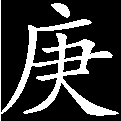
\includegraphics[width=3mm]{../Images/00004}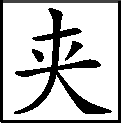
\includegraphics[width=3mm]{../Images/00012}\footnotesize \kaishu 纯写阿凤以衬后文,二人形景如见,语言如闻,真描画的到。}

说着,早已合算了,共凑了一百五十两有馀。贾母道:``一日戏酒用不了。''尤氏道:``既不请客,酒席又不多,两三日的用度都够了。头等,戏不用钱,省在这上头。''贾母道:``凤丫头说那一班好,就传那一班。''凤姐儿道:``咱们家的班子都听熟了,倒是花几个钱叫一班来听听罢。''贾母道:``这件事我交给珍哥媳妇了。越性叫凤丫头别操一点心,受用一日才算。''{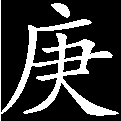
\includegraphics[width=3mm]{../Images/00004}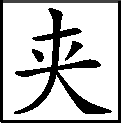
\includegraphics[width=3mm]{../Images/00012}\footnotesize \kaishu 所以特受用了,才有琏卿之变。乐极生悲,自然之理。}尤氏答应着。又说了一回话,都知贾母乏了,才渐渐的都散出来。

尤氏等送邢夫人王夫人二人散去,便往凤姐房里来商议怎么办生日的话。凤姐儿道:``你不用问我,你只看老太太的眼色行事就完了。''尤氏笑道:``你这阿物儿,也忒行了大运了。我当有什么事叫我们去,原来单为这个。出了钱不算,还要我来操心,你怎么谢我?''凤姐笑道:``你别扯臊,我又没叫你来,谢你什么!你怕操心?你这会子就回老太太去,再派一个就是了。''尤氏笑道:``你瞧他兴的这样儿!我劝你收着些儿好。太满了就泼出来了。''二人又说了一回方散。

次日将银子送到宁国府来,尤氏方才起来梳洗,因问是谁送过来的,丫鬟们回说:``是林大娘。''尤氏便命叫了他来。丫鬟走至下房,叫了林之孝家的过来。尤氏命他脚踏上坐了,一面忙着梳洗,一面问他:``这一包银子共多少?''林之孝家的回说:``这是我们底下人的银子,凑了先送过来。老太太和太太们的还没有呢。''正说着,丫鬟们回说:``那府里太太和姨太太打发人送分子来了。''尤氏笑骂道:``小蹄子们,专会记得这些没要紧的话。昨儿不过老太太一时高兴,故意的要学那小家子凑分子,你们就记得,到了你们嘴里当正经的说。{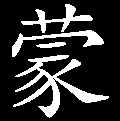
\includegraphics[width=3mm]{../Images/00006}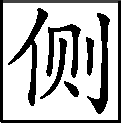
\includegraphics[width=3mm]{../Images/00011}\footnotesize \kaishu 世家风调。}还不快接了进来好生待茶,再打发他们去。''丫鬟应着,忙接了进来,一共两封,连宝钗黛玉的都有了。尤氏问还少谁的,林之孝家的道:``还少老太太、太太、姑娘们的和底下姑娘们的。''尤氏道:``还有你们大奶奶的呢?''林之孝家的道:``奶奶过去,这银子都从二奶奶手里发,{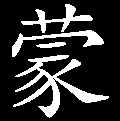
\includegraphics[width=3mm]{../Images/00006}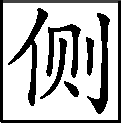
\includegraphics[width=3mm]{../Images/00011}\footnotesize \kaishu 伏线。}一共都有了。''

说着,尤氏已梳洗了,命人伺候车辆。一时来至荣府,先来见凤姐。只见凤姐已将银子封好,正要送去。尤氏问:``都齐了?''凤姐儿笑道:{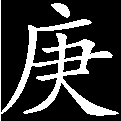
\includegraphics[width=3mm]{../Images/00004}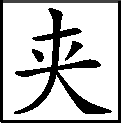
\includegraphics[width=3mm]{../Images/00012}\footnotesize \kaishu ``笑''字就有神情。}``都有了,快拿了去罢,丢了我不管。''{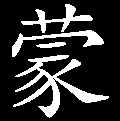
\includegraphics[width=3mm]{../Images/00006}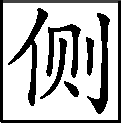
\includegraphics[width=3mm]{../Images/00011}\footnotesize \kaishu {(斗)}{[}逗{]}起。}尤氏笑道:``我有些信不及,倒要当面点一点。''说着果然按数一点,只没有李纨的一分。{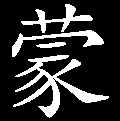
\includegraphics[width=3mm]{../Images/00006}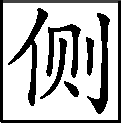
\includegraphics[width=3mm]{../Images/00011}\footnotesize \kaishu 点明题面。}尤氏笑道:``我说你肏鬼呢,怎么你大嫂子的没有?''凤姐儿笑道:``那么些还不够使?短一分儿也罢了,等不够了我再给你。''{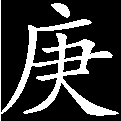
\includegraphics[width=3mm]{../Images/00004}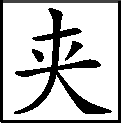
\includegraphics[width=3mm]{../Images/00012}\footnotesize \kaishu 可见阿凤处处心机。}尤氏道:``昨儿你在人跟前作人,今儿又来和我赖,这个断不依你。我只和老太太要去。''凤姐儿笑道:``我看你利害。明儿有了事,我也`丁是丁卯是卯'的,你也别抱怨。''尤氏笑道:``你一般的也怕。不看你素日孝敬我,我才是不依你呢。''{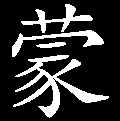
\includegraphics[width=3mm]{../Images/00006}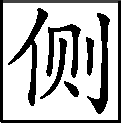
\includegraphics[width=3mm]{../Images/00011}\footnotesize \kaishu 处处是世情作趣,处处是随笔埋伏。}说着,把平儿的一分拿了出来,说道:``平儿,来!把你的收起去,等不够了,我替你添上。''平儿会意,因说道:``奶奶先使着,若剩下了再赏我一样。''尤氏笑道:``只许你那主子作弊,就不许我作情儿。''{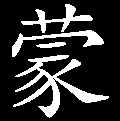
\includegraphics[width=3mm]{../Images/00006}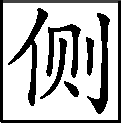
\includegraphics[width=3mm]{../Images/00011}\footnotesize \kaishu 请看。}平儿只得收了。尤氏又道:``我看着你主子这么细致,弄这些钱那里使去!使不了,明儿带了棺材里使去。''{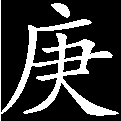
\includegraphics[width=3mm]{../Images/00004}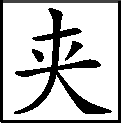
\includegraphics[width=3mm]{../Images/00012}\footnotesize \kaishu 此言不假,伏下后文短命。尤氏亦能干事矣,惜不能劝夫治家,惜哉痛哉!}

一面说着,一面又往贾母处来。先请了安,大概说了两句话,便走到鸳鸯房中和鸳鸯商议,只听鸳鸯的主意行事,何以讨贾母的喜欢。二人计议妥当。尤氏临走时,也把鸳鸯二两银子还他,{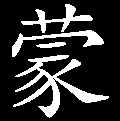
\includegraphics[width=3mm]{../Images/00006}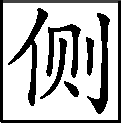
\includegraphics[width=3mm]{../Images/00011}\footnotesize \kaishu 请看世情。可笑可笑!}说:``这还使不了呢。''说着,一径出来,又至王夫人跟前说了一回话。因王夫人进了佛堂,把彩云的一分也还了他。见凤姐不在跟前,一时把周、赵二人的也还了。{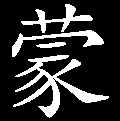
\includegraphics[width=3mm]{../Images/00006}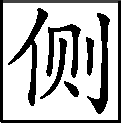
\includegraphics[width=3mm]{../Images/00011}\footnotesize \kaishu 另是一番作用。}他两个还不敢收。{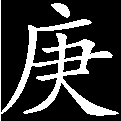
\includegraphics[width=3mm]{../Images/00004}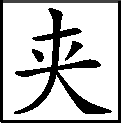
\includegraphics[width=3mm]{../Images/00012}\footnotesize \kaishu 阿凤声势亦甚矣。}尤氏道:``你们可怜见的,那里有这些闲钱?凤丫头便知道了,有我应着呢。''二人听说,千恩万谢的方收了。{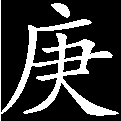
\includegraphics[width=3mm]{../Images/00004}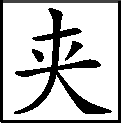
\includegraphics[width=3mm]{../Images/00012}\footnotesize \kaishu 尤氏亦可谓有才矣。论有德比阿凤高十倍,惜乎不能谏夫治家,所谓``人各有当''也。此方是至理至情,最恨近之野史中,恶则无往不恶,美则无一不美,何不近情理之如是耶?}\href{../Text/part0047_split_000.html\#lnkback_1_a}{\textsuperscript{①}}

展眼已是九月初二日,园中人都打听得尤氏办得十分热闹,{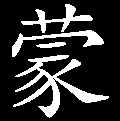
\includegraphics[width=3mm]{../Images/00006}\includegraphics[width=3mm]{../Images/00011}\footnotesize \kaishu 剩笔,且影射能事不独熙凤。}不但有戏,连耍百戏并说书的男女先儿全有,都打点取乐顽耍。李纨又向众姊妹道:``今儿是正经社日,可别忘了。{\includegraphics[width=3mm]{../Images/00004}\includegraphics[width=3mm]{../Images/00012}\footnotesize \kaishu 看书者已忘,批书者亦已忘了,作者竟未忘。忽写此事,真忙中愈忙、紧处愈紧也。}宝玉也不来,想必他只图热闹,把清雅就丢开了。''{\includegraphics[width=3mm]{../Images/00004}\includegraphics[width=3mm]{../Images/00012}\footnotesize \kaishu 此独宝玉乎?亦骂世人。余亦谓宝玉忘了,不然何不来耶?}说着,便命丫鬟去瞧作什么,快请了来。丫鬟去了半日,回说:``花大姐姐说,今儿一早就出门去了。''{\includegraphics[width=3mm]{../Images/00004}\includegraphics[width=3mm]{../Images/00012}\footnotesize \kaishu 奇文。}众人听了,都诧异说:``再没有出门之理。这丫头糊涂,不知说话。''因又命翠墨去。

一时翠墨回来说:``可不真出了门了。说有个朋友死了,出去探丧去了。''{\includegraphics[width=3mm]{../Images/00004}\includegraphics[width=3mm]{../Images/00012}\footnotesize \kaishu 奇文。信有之乎?花团锦簇之日偏如此写法。}探春道:``断然没有的事。凭他什么,再没今日出门之理。你叫袭人来,我问他。''刚说着,只见袭人走来。李纨等都说道:``今儿凭他有什么事,也不该出门。头一件,你二奶奶的生日,老太太都这等高兴,两府上下众人来凑热闹,他倒走了;{\includegraphics[width=3mm]{../Images/00006}\includegraphics[width=3mm]{../Images/00011}\footnotesize \kaishu 因行文不肯平,下一反笔,则文语并奇,好看煞人。}第二件,又是头一社的正日子,他也不告假,就私自去了!''袭人叹道:``昨儿晚上就说了,今儿一早起有要紧的事到北静王府里去,就赶回来的。劝他不要去,他必不依。今儿一早起来,又要素衣裳穿,想必是北静王府里的要紧姬妾没了,也未可知。''李纨等道:``若果如此,也该去走走,只是也该回来了。''说着,大家又商议:``咱们只管作诗,等他回来罚他。''刚说着,只见贾母已打发人来请,便都往前头来了。袭人回明宝玉的事,贾母不乐,便命人去接。

原来宝玉心里有件私事,于头一日就吩咐茗烟:``明日一早要出门,备下两匹马在后门口等着,不要别一个跟着。说给李贵,我往北府里去了。倘或要有人找我,叫他拦住不用找,只说北府里留下了,横竖就来的。''茗烟也摸不着头脑,只得依言说了。今儿一早,果然备了两匹马在园后门等着。天亮了,只见宝玉遍体纯素,从角门出来,一语不发跨上马,一弯腰,顺着街就颠下去了。茗烟也只得跨马加鞭赶上,在后面忙问:``往那里去?''宝玉道:``这条路是往那里去的?''茗烟道:``这是出北门的大道。出去了冷清清没有可顽的。''宝玉听说,点头道:``正要冷清清的地方好。''说着,越性加了鞭,那马早已转了两个弯子,出了城门。茗烟越发不得主意,只得紧紧跟着。

一气跑了七八里路出来,人烟渐渐稀少,宝玉方勒住马,回头问茗烟道:``这里可有卖香的?''茗烟道:``香倒有,不知是那一样?''宝玉想道:``别的香不好,须得檀、芸、降三样。''茗烟笑道:``这三样可难得。''宝玉为难。茗烟见他为难,因问道:``要香作什么使?我见二爷时常小荷包有散香,何不找一找。''一句提醒了宝玉,便回手向衣襟上拉出一个荷包来,摸了一摸,竟有两星沉速,心内欢喜:``只是不恭些。''再想自己亲身带的,倒比买的又好些。于是又问炉炭。茗烟道:``这可罢了。荒郊野外那里有?用这些何不早说,带了来岂不便宜。''宝玉道:``糊涂东西,若可带了来,又不这样没命的跑了。''{\includegraphics[width=3mm]{../Images/00004}\includegraphics[width=3mm]{../Images/00012}\footnotesize \kaishu 奇奇怪怪,不知为何?看他下文怎样。}

茗烟想了半日,笑道:``我得了个主意,不知二爷心下如何?我想二爷不只用这个呢,只怕还要用别的。这也不是事。如今我们往前再走二里地,就是水仙庵了。''宝玉听了忙问:``水仙庵就在这里?更好了,我们就去。''说着,就加鞭前行,一面回头向茗烟道:``这水仙庵的姑子长往咱们家去,咱们这一去到那里,和他借香炉使使,他自然是肯的。''茗烟道:``别说他是咱们家的香火,就是平白不认识的庙里,和他借,他也不敢驳回。只是一件,我常见二爷最厌这水仙庵的,如何今儿又这样喜欢了?''宝玉道:``我素日因恨俗人不知原故,混供神混盖庙,这都是当日有钱的老公们和那些有钱的愚妇们听见有个神,就盖起庙来供着,也不知那神是何人,因听些野史小说,便信真了。{\includegraphics[width=3mm]{../Images/00004}\includegraphics[width=3mm]{../Images/00012}\footnotesize \kaishu 近闻刚丙庙,又有三教庵,以如来为尊,太上为次,先师为末,真杀有馀辜,所谓此书救世之溺不假。}比如这水仙庵里面因供的是洛神,故名水仙庵,殊不知古来并没有个洛神,那原是曹子建的谎话,谁知这起愚人就塑了像供着。今儿却合我的心事,故借他一用。''

说着早已来至门前。那老姑子见宝玉来了,事出意外,竟像天上掉下个活龙来的一般,忙上来问好,命老道来接马。宝玉进去,也不拜洛神之像,却只管赏鉴。虽是泥塑的,却真有``翩若惊鸿,婉若游龙''之态,``荷出绿波,日映朝霞''之姿。{\includegraphics[width=3mm]{../Images/00004}\includegraphics[width=3mm]{../Images/00012}\footnotesize \kaishu 妙极!用《洛神赋》赞洛神,本地风光,愈觉新奇。}宝玉不觉滴下泪来。老姑子献了茶。宝玉因和他借香炉。那姑子去了半日,连香供纸马都预备了来。宝玉道:``一概不用。''说着,命茗烟捧着炉出至后园中,拣一块干净地方儿,竟拣不出。茗烟道:``那井台儿上如何?''宝玉点头,一齐来至井台上,将炉放下。{\includegraphics[width=3mm]{../Images/00004}\includegraphics[width=3mm]{../Images/00012}\footnotesize \kaishu 妙极之文。宝玉心中拣定是井台上了,故意使茗烟说出,使彼不犯疑猜矣。宝玉亦有欺人之才,盖不用耳。}

茗烟站过一旁。宝玉掏出香来焚上,含泪施了半礼,{\includegraphics[width=3mm]{../Images/00004}\includegraphics[width=3mm]{../Images/00012}\footnotesize \kaishu 奇文。云``只施半礼'',终不知为何事也。}回身命收了去。茗烟答应,且不收,忙爬下磕了几个头,口内祝道:``我茗烟跟二爷这几年,二爷的心事,我没有不知道的,只有今儿这一祭祀没有告诉我,我也不敢问。只是这受祭的阴魂虽不知名姓,想来自然是那人间有一、天上无双,极聪明极俊雅的一位姐姐妹妹了。二爷心事不能出口,让我代祝:若芳魂有感,香魄多情,虽然阴阳间隔,既是知己之间,时常来望候二爷,未尝不可。你在阴间保佑二爷来生也变个女孩儿,和你们一处相伴,再不可又托生这须眉浊物了。''说毕,又磕几个头,才爬起来。{\includegraphics[width=3mm]{../Images/00004}\includegraphics[width=3mm]{../Images/00012}\footnotesize \kaishu 忽插入茗烟一篇流言,粗看则小儿戏语,亦甚无味。细玩则大有深意。试思宝玉之为人,岂不应有一极伶俐乖巧小童哉?此一祝亦如《西厢记》中双文降香,第三炷则不语,红娘则代祝数语,直将双文心事道破。此处若写宝玉一祝,则成何文字?若不祝则成一哑谜,如何散场?故写茗烟一戏,直戏入宝玉心中,又发出前文,又可收后文,又写茗烟素日之乖觉可人,且衬出宝玉直似一个守礼待嫁的女儿一般,其素日脂香粉气不待写而全现出矣。今看此回,直欲将宝玉当作一个极清俊羞怯的女儿,看茗烟则极乖觉可人之丫鬟也。}

宝玉听他没说完,便撑不住笑了,{\includegraphics[width=3mm]{../Images/00004}\includegraphics[width=3mm]{../Images/00012}\footnotesize \kaishu 方一笑,盖原可发笑,且说的合心,愈见可笑也。}因踢他道:``休胡说,看人听见笑话。''{\includegraphics[width=3mm]{../Images/00004}\includegraphics[width=3mm]{../Images/00012}\footnotesize \kaishu 也知人笑,更奇。}茗烟起来收过香炉,和宝玉走着,因道:``我已经和姑子说了,二爷还没用饭,叫他随便收拾了些东西,二爷勉强吃些。我知道今儿咱们里头大排筵宴,热闹非常,二爷为此才躲了出来的。横竖在这里清净一天,也就尽到礼了。若不吃东西,断使不得。''宝玉道:``戏酒既不吃,这随便素的吃些何妨。''茗烟道:``这便才是。还有一说,咱们来了,还有人不放心。若没有人不放心,便晚了进城何妨?若有人不放心,二爷须得进城回家去才是。第一老太太、太太也放了心,第二礼也尽了,不过如此。就是家去了看戏吃酒,也并不是二爷有意,原不过陪着父母尽孝道。二爷若单为了这个,不顾老太太、太太悬心,就是方才那受祭的阴魂也不安生。二爷想我这话如何?''宝玉笑道:``你的意思我猜着了,你想着只你一个跟了我出来,回来你怕担不是,所以拿这大题目来劝我。{\includegraphics[width=3mm]{../Images/00004}\includegraphics[width=3mm]{../Images/00012}\footnotesize \kaishu 亦知这个大,妙极!}我才来了,不过为尽个礼,再去吃酒看戏,并没说一日不进城。这已完了心愿,赶着进城,大家放心,岂不两尽其道。''{\includegraphics[width=3mm]{../Images/00004}\includegraphics[width=3mm]{../Images/00012}\footnotesize \kaishu 这是大通的意见,世人不及的去处。}茗烟道:``这更好了。''说着二人来至禅堂,果然那姑子收拾了一桌素菜,宝玉胡乱吃了些,茗烟也吃了。

二人便上马仍回旧路。茗烟在后面只嘱咐:``二爷好生骑着,这马总没大骑的,手里提紧着。''{\includegraphics[width=3mm]{../Images/00004}\includegraphics[width=3mm]{../Images/00012}\footnotesize \kaishu 看他偏不写凤姐那样热闹,却写这般清冷,真世人意料不到这一篇文字也。}一面说着,早已进了城,仍从后门进去,忙忙来至怡红院中。袭人等都不在房里,只有几个老婆子看屋子,见他来了,都喜的眉开眼笑,说:``阿弥陀佛,可来了!把花姑娘急疯了!上头正坐席呢,二爷快去罢。''宝玉听说忙将素服脱了,自去寻了华服换上,问在什么地方坐席,老婆子回说在新盖的大花厅上。

宝玉听说,一径往花厅来,耳内早已隐隐闻得歌管之声。刚至穿堂那边,只见玉钏儿独坐在廊檐下垂泪,{\includegraphics[width=3mm]{../Images/00004}\includegraphics[width=3mm]{../Images/00012}\footnotesize \kaishu 总是千奇百怪的文字。}一见他来,便收泪说道:``凤凰来了,快进去罢。再一会子不来,都反了。''{\includegraphics[width=3mm]{../Images/00004}\includegraphics[width=3mm]{../Images/00012}\footnotesize \kaishu 是平常言语,却是无限文章,无限情理。看至后文,再细思此言,则可知矣。}宝玉陪笑道:``你猜我往那里去了?''玉钏儿不答,只管擦泪。{\includegraphics[width=3mm]{../Images/00004}\includegraphics[width=3mm]{../Images/00012}\footnotesize \kaishu 无限情理。}宝玉忙进厅里,见了贾母王夫人等,众人真如得了凤凰一般。

宝玉忙赶着与凤姐儿行礼。贾母王夫人都说他不知道好歹,``怎么也不说声就私自跑了,这还了得!明儿再这样,等老爷回家来,必告诉他打你。''说着又骂跟的小厮们都偏听他的话,说那里去就去,也不回一声儿。一面又问他到底那去了,可吃了什么,可唬着了。{\includegraphics[width=3mm]{../Images/00004}\includegraphics[width=3mm]{../Images/00012}\footnotesize \kaishu 奇文,毕肖。}宝玉只回说:``北静王的一个爱妾昨日没了,给他道恼去。他哭的那样,不好撇下就回来,所以多等了一会子。''贾母道:``以后再私自出门,不先告诉我们,一定叫你老子打你。''宝玉答应着。因又要打跟的小子们,众人又忙说情,又劝道:``老太太也不必过虑了,他已经回来,大家该放心乐一回了。''贾母先不放心,自然发狠,如今见他来了,喜且有馀,那里还恨,也就不提了;还怕他不受用,或者别处没吃饱,路上着了惊怕,反百般的哄他。袭人早过来伏侍。大家仍旧看戏。当日演的是《荆钗记》,贾母薛姨妈等都看的心酸落泪,也有叹的,也有骂的。要知端的,下回分解。

{\includegraphics[width=3mm]{../Images/00005} \kaishu 总评:攒金办寿家常乐,素服焚香无限情。}

{写办事不独熙凤,写多情不漏亡人,情之所钟必让若辈。此所谓``情情''者也。}

{\href{../Text/part0047_split_000.html\#navto_1_a}{①}此后戚、蒙本多``于是尤氏一径出来,坐车回家。不在话下。且说''一十八字。}
